%! Author = saya
%! Date = 9/19/2023

\section{History of errors and failures in electronic systems}
\label{sec:history-errors-failures-in-electronic-systems}
%%%%%%%%%%%%%%%%%%%%%%%%%%%%%%%%%%%%%%%%%%%%%%%%%%%%%%%%%%%%%%%%%%%%%%%%%%%%%%%%

\subsection{Electronics-related failures in avionic systems}
\label{subsec:elec-failres-in-avionics}

According to field surveys published by the \ac{FAA} and \ac{NTSB}, a total
of 24\% of failures in the aviation industry were caused by faulty subsystems,
and up to 26\% of loss of control cases were directly attributed to
hardware failure~\autocite{belcastro}.
Lethal accidents in commercial airlines during the period between 1987 and 2005
were generally caused by:

\begin{itemize}[topsep=8pt,itemsep=4pt,partopsep=4pt, parsep=4pt]
    \item \ac{CFIT}
    \item loss-of-control in flight
    \item system/component failure or malfunction
\end{itemize}

While the controlled flight into terrain has been dealt with to some degree by
adding safeguard measures, accidents due to system/component and software
failures are still a point of concern.
As it can be seen in \autoref{fig:aircraft-incidents}, based on a field survey
in military aviation, the majority of hardware failures in electronic systems
of military aviation were caused by interconnection
failures~\autocite{norton-mishap} while discrete component failures have
the lowest contribution, yet they are still a considerable risk, because
more components introduce more failures.
One reason for the low percentage of the failure rate could be that the
materials used in \ac{PCB} and electronic components are less likely to survive
a crash event. In such scenarios, the damage can prevent the components from
being identified as failure causes or even be considered as having a role in
the mishap~\autocite{Galler}.

\begin{figure}[h]
    \centering
    \begin{tikzpicture}
        \pie[
%            color={black!10, black!20, black!30, black!40, black!50},
            pos={0, 0},
            text=legend, style=drop shadow, radius=2]
        {
            36/Interconnections,
            26/Instruments,
            25/Power Systems,
            10/Electromechanical Devices,
            3/Passive Components
        }
    \end{tikzpicture}
    \caption[Summary electrical related aircraft incidents]{Summary of
    electrically related aircraft incidents, according to a database of Norton
    Airforce Base \autocite{norton-mishap}}
    \label{fig:aircraft-incidents}
\end{figure}

\begin{figure}[h]
    \centering
    \begin{tikzpicture}
        \pie[
%            color={black!10, black!20, black!30, black!40},
            pos={0, 0},
            text=legend, style=drop shadow, radius=2]
        {
            40/Connections,
            30/Parts on PCBs,
            20/Connections on PCBs,
            10/Other
        }
    \end{tikzpicture}
    \caption[Causes of aircraft equipment failure]{Causes of aircraft
    equipment failures according to data from the
    Avionics Integrity Program~\autocite{halpin}.}
    \label{fig:aircraft-equipmentfailure}
\end{figure}

\autoref{fig:aircraft-equipmentfailure} represents a detailed look into aircraft
electronic equipment failures, identifying interconnects on
circuit boards (trace and via connections) as significant reasons for
mishaps\autocite{halpin}.

A survey based on reported repair cases of 58,000 faulty electronic equipment
modules with different complexity and service lifetime indicate that passive
and active components are major causes of failure \autocite{wong1987culprits}
as it can be seen in \autoref{fig:aircraft-component-errors}.

While it is unlikely that a single component can be the sole reason for an
airplane crash, as the standards dictate the availability of redundancy for
critical systems, selecting the suitable component for the proper mission
profile should not be underestimated.

A survey in Hughes Aircraft Factory \autocite{Galler} concludes that:

\begin{enumerate}[topsep=8pt,itemsep=4pt,partopsep=4pt, parsep=4pt]
    \item Most of the aircraft mishaps in electronic equipment are attributed to
    interconnection problems (wiring and connectors) at the sub-system level due
    to electrical arcing and corrosion, breakdown of insulation stability due to
    aging, or broken connectors.
    \item Passive and active components are primarily responsible for electronic
    equipment failures on \ac{PCB} level.
\end{enumerate}

The aviation industry follows high safety and reliability standards, and
redundancy of critical systems is enforced by standards such that one component
(single point of failure) should never lead to a catastrophe.

\begin{figure}[h]
    \centering
    \settowidth{\TL}{\footnotesize Integrated}
    \begin{tikzpicture}
        \begin{axis}[
            width = \linewidth,
            symbolic x coords = {Integrated Circuits, Transistors, Capacitors,
            Resistors, Hybrid Circuits, Diodes, Others,
            Solder Joints},
            bar width=6.8mm,
            ybar,
            xtick=data,
            enlarge x limits=0.08,
            ticklabel style = {font=\footnotesize\linespread{0.76}\relax,
            inner ysep=0pt},
            xticklabel style = {text width=\TL, align=right,
            anchor=north east, rotate=30},
            legend entries={Percentage of replacement}
        ]
            \addplot coordinates {
                (Integrated Circuits,   27)
                (Transistors,           14)
                (Capacitors,            12)
                (Resistors,             12)
                (Hybrid Circuits,       12)
                (Diodes,                10)
                (Others,                10)
                (Solder Joints,         3)
            };
        \end{axis}
    \end{tikzpicture}

    \caption[Most replaced items in avionic repairs]{Most replaced items in
    \ac{PCB} based on data from Hughes Aircraft Factory
    \autocite{wong1987culprits}.}
    \label{fig:aircraft-component-errors}
\end{figure}

\

%%%% Automotive %%%%%%%%%%%%%%%%%%%%%%%%%%%%%%%%%%%%%%%%%%%%%%%%%%%%%%%%%%%%%%%%

\subsection{Electronics-related failures in automotive systems}
\label{subsec:elec-failures-in-automotive}

While the aviation industry has a long history of employing electronic
equipment, the automotive industry is a newcomer to electric circuits.

For a major part of the last century, cars and trucks were operated from
mechanical and hydraulic systems.
It was not before the last decades of the previous century that the industry
shifted to electronic equipment to improve control systems in cars.
Sophisticated \acp{ECU} are playing a significant role in
the automotive industry, mainly because of major advancements in the
semiconductor industry (smart power).

A modern car is equipped with many \ac{ECU}s~(\autoref{fig:ecu-open}) with
safety-critical tasks, from engine control (e.g. ignition), \ac{ABS},
\ac{ESP} to fully automated driving with all its near-neighborhood analysis
tools (Lidar, Radar, etc.).

\begin{figure}[t]
    \centering
    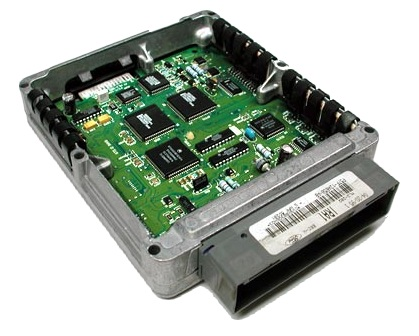
\includegraphics[scale=0.5]
    {figures/ecu-open.jpg}
    \caption[Inside of a modern ECU]{Inside of a modern \ac{ECU} where
    integrated circuits and passive components are carried on a \ac{PCB}.}
    \label{fig:ecu-open}
\end{figure}

Automotive-grade \acp{ECU} are similar in structure compared to aviation
equipment: The modules have a well-defined task realized with passive and
active components, connectors and interconnects, assembled on multi-layer
carrier boards referred to as \ac{PCB} or \ac{PWB}.
Consequently, modern \ac{ECU} in automotive applications are comparable to their
counterparts in aviation industry, they go through the same intensive tests and
qualification programs before being commissioned for public service.

Although there are different types of stress for airborne and ground-based
transportation systems (cars, trains), unprotected failures result in accidents.
Therefore, it is vital to test and qualify all components and building blocks to
define the lifespan and fitness of these electronic systems.

%%%% Madical %%%%%%%%%%%%%%%%%%%%%%%%%%%%%%%%%%%%%%%%%%%%%%%%%%%%%%%%%%%%%%%%%%%

\subsection{Electronics-related failures in medical systems}
\label{subsec:elec-failures-in-medical}

Medical equipment is another major safety-critical category of electronic
systems.
Such devices are used extensively in operation rooms and intensive care
stations in hospitals or patient homes. Just like aviation and automotive
electronic systems, these medical-grade devices are made of passive and active
components interconnected on a \ac{PCB}, making them susceptible to similar
defects and failure modes.

The rising number of older adults gave the medical industry rapid growth as more
medical devices are required to support this trend \autocite{hedge}.
Medical devices rely on electronic components and integrated circuits, and we
have another safety-critical group of systems where small failures severely
impact users.
Proper testing of all components and systems is utterly critical.

The \ac{FDA} medical device recall database is a source of knowledge for failure
rates in electronic systems.
This database contains all failure records since November 2002.
It unveils problems affecting medical devices at the board level and
component level, which can be advantageous for future mitigations and
preventive measures \autocite{fda-med-recalls}.

Just between the years 2006 and 2011, the FDA has reported 5,294 recalls and
1,154,451 adverse incidents caused by electronic medical
devices \autocite{alemzadeh}.
\autoref{fig:fda-data} shows a clear uptrend in the number of incidents year
over year, stressing the fact that test methods and test equipment must be
reassessed and brought up to date.

\begin{figure}[ht]
    \centering

    \resizebox{\linewidth}{!}{%
    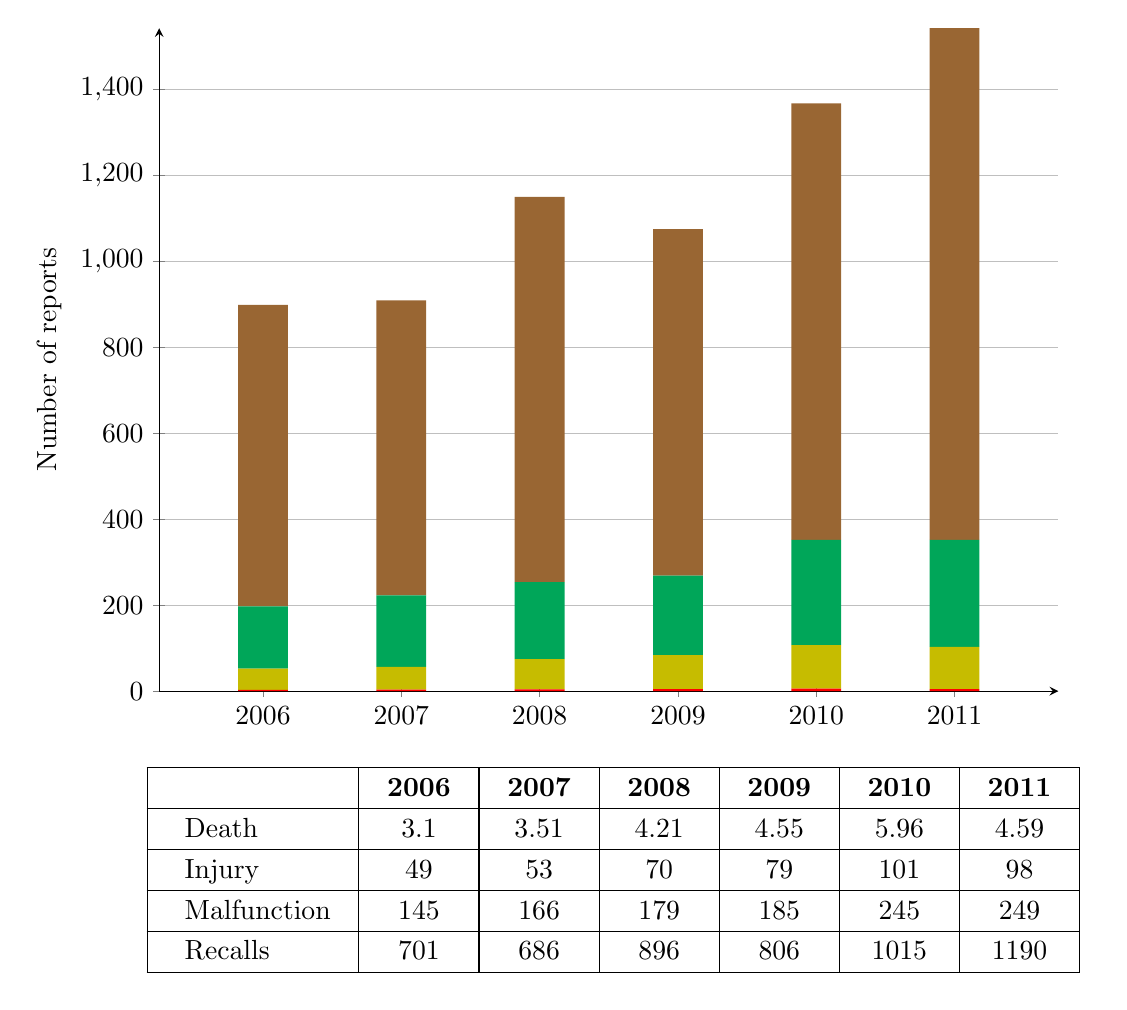
\begin{tikzpicture}
        \begin{axis}[
            ybar stacked,
            bar width=18pt,
            width=13cm,
            height=10cm,
            symbolic x coords={2006,2007,2008,2009,2010,2011},
            xtick=data,
            ylabel={Number of reports},
            ymin=0,
            axis lines=left,
            ymajorgrids,
            enlarge x limits=0.15,
            clip=false,
            legend style={
                at={(0.5,1.05)},
                anchor=south,
                legend columns=4
            }
        ]
% --- stacked bars ---
            \addplot[fill=red, draw=none]
            coordinates {(2006,3.1) (2007,3.51) (2008,4.21) (2009,4.55) (2010,5.96) (2011,4.59)};

            \addplot[fill=olive!50!yellow, draw=none]
            coordinates {(2006,49) (2007,53) (2008,70) (2009,79) (2010,101) (2011,98)};

            \addplot[fill=green!30!teal, draw=none]
            coordinates {(2006,145) (2007,166) (2008,179) (2009,185) (2010,245) (2011,249)};

            \addplot[fill=brown!80!black, draw=none]
            coordinates {(2006,701) (2007,686) (2008,896) (2009,806) (2010,1015) (2011,1190)};

            %\legend{Death, Injury, Malfunction, Recalls}

% --- table under the plot ---
            \node[
                anchor=north,
                align=center
            ] at (axis description cs:0.5,-0.1) {

                \setlength{\tabcolsep}{10pt}
                \renewcommand{\arraystretch}{1.2}
                \begin{tabular}{|l|c|c|c|c|c|c|}
                    \hline
                    & \textbf{2006} & \textbf{2007} & \textbf{2008} & \textbf{2009} & \textbf{2010} & \textbf{2011} \\
                    \hline
                    {\color{red}$\blacksquare$} Death
                    & 3.1 & 3.51 & 4.21 & 4.55 & 5.96 & 4.59 \\
                    \hline
                    {\color{olive!50!yellow}$\blacksquare$} Injury
                    & 49 & 53 & 70 & 79 & 101 & 98 \\
                    \hline
                    {\color{green!30!teal}$\blacksquare$} Malfunction
                    & 145 & 166 & 179 & 185 & 245 & 249 \\
                    \hline
                    {\color{brown!80!black}$\blacksquare$} Recalls
                    & 701 & 686 & 896 & 806 & 1015 & 1190 \\
                    \hline
                \end{tabular}
            };

        \end{axis}
    \end{tikzpicture}
    }

    \caption[\acs{FDA} Medical device issues between 2006 and 2011]{
        Hardware and software-related failures for medical devices,
        including adverse consequences (in thousands)
        \autocite{alemzadeh}.}
    \label{fig:fda-data}
\end{figure}

%%%% Consumer %%%%%%%%%%%%%%%%%%%%%%%%%%%%%%%%%%%%%%%%%%%%%%%%%%%%%%%%%%%%%%%%%%



\subsection{Electronics-related failures in consumer products}
\label{subsec:elec-failures-in-consumer}

On the consumer side, we have observed an increase in the use of electronic
devices since the middle of the last century.
The introduction of radio and television units started this development,
followed by the introduction of home computers and mobile phones.
The complexity of today’s consumer electronics is not much less than what was
available in military aircraft and satellites just a few years ago.

Unlike aviation, automotive, or medical industries, the consumer electronics
industry is a \enquote{high-volume, low-margin} \autocite{Mozar}
market that puts design and production chains under pressure to achieve the
highest possible profit margins. Consumer products need to be safe and reliable as well.
Nobody could accept that mobile phone or laptop batteries burst in flames due to
unreliable and improper battery or charging circuit design or components
(\autoref{fig:eswollen-battery}).
Therefore, the safety of consumer electronics must be ensured to reduce the
number of incidents \autocite{Harada}.

\begin{figure}[t]
    \centering
    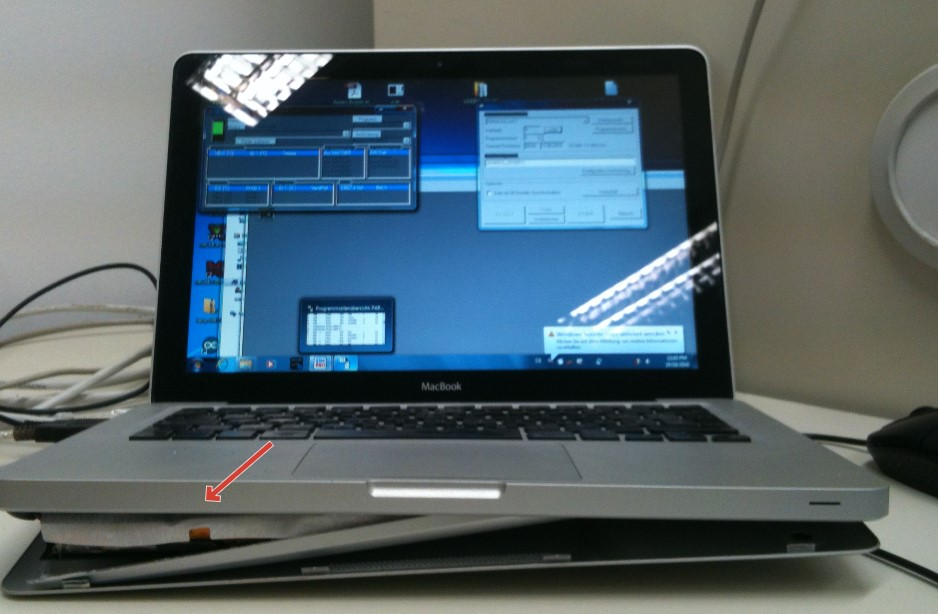
\includegraphics[scale=0.3]
    {figures/swollen-laptop-battery_jpg}
    \caption[Swollen Lithium-ion Battery]{A Consumer-grade laptop
    with lithium-ion battery expanded due to a short circuit failure.}
    \label{fig:eswollen-battery}
\end{figure}

There are many more examples, and all of them bring us to the fact that
electronic systems must be as safe and reliable as possible and be qualified
to operate under their given mission profile.
